This section outlines the architectural strategy for the flow of the RV8 work cell system, defining the top-level logical view of the design. The system is structured into three distinct layers: Input, Processing, and Output. Each of these layers serves a specific and vital function within the system, enabling the robot to perform fixed tasks based on the program. This section includes a high-level block diagram that visually illustrates the relationships and interactions between these layers, providing a comprehensive overview of the system's architecture.  

\begin{figure}[h!]
	\centering
 	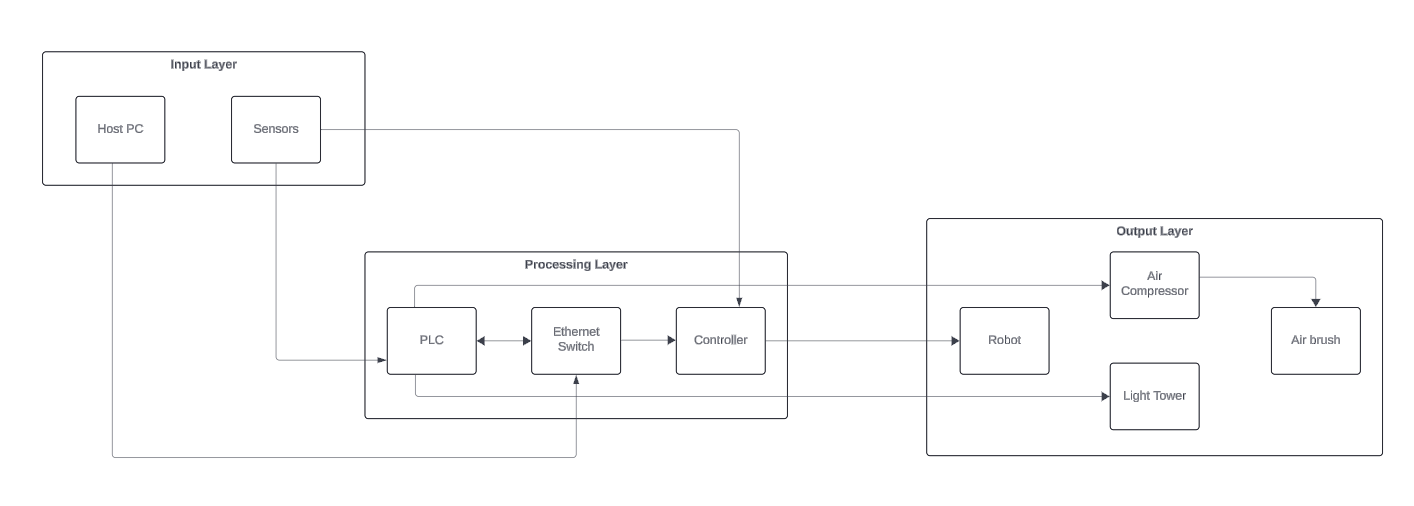
\includegraphics[width=1\textwidth]{images/System_sub.png}
 \caption{System architecture}
\end{figure}
